\level{1}{Design Patterns} \label{app:designpattern}
	\level{2}{Model View Controller} \label{app:MVC}
		\begin{figure}[H]\centering
        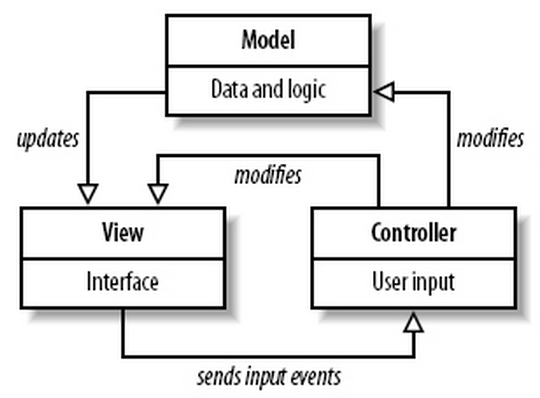
\includegraphics[scale=0.7]{SpecificaTecnica/Pics/MVC}
        \caption{Struttura del pattern Model View Controller}
		\end{figure}
		Model-View-Controller (\insglo{MVC}) è un \insglo{pattern} architetturale utilizzato per dividere il codice in blocchi di funzionalità ben distinte, e viene utilizzato molto frequentemente nelle applicazioni in cui un insieme di informazioni deve essere rappresentato attraverso una interfaccia grafica.
		\level{3}{Componenti}
			\insglo{MVC} è quindi basato sul principio del disaccoppiamento dei tre oggetti di cui è composto, ovvero sulla riduzione del loro grado di dipendenza reciproca, allo scopo di fornire una maggiore robustezza, modularità e manutenibilità al \insglo{software}.\\
			Di seguito si riporta una breve descrizione dei componenti e delle loro caratteristiche. 
			\level{4}{Model}
				Il Model è il nucleo dell'applicazione. Definisce il modello dei dati realizzando la business logic, ovvero definisce gli oggetti secondo la logica di utilizzo dell'applicazione indicante anche le possibili operazioni effettuabili su di essi.\\
				Questo componente viene generalmente progettato attraverso tecniche object oriented.\\
				Nella struttura del \insglo{pattern} \insglo{MVC}, il Model è un componente passivo, che non ha relazioni uscenti forti, ma si occupa di notificare alla View eventuali aggiornamenti avvenuti in esso, solitamente attraverso l'implementazione del \insglo{pattern} Observer.
			\level{4}{View}
				La View si occupa di visualizzare i dati contenuti nel Model e fornisce l'interfaccia di interazione con utenti e agenti.\\
				Nella struttura del \insglo{pattern} \insglo{MVC}, la View cattura gli input dell'utente e li passa al Controller affinché esegua le corrette operazioni sul Model. \\
				La View può essere soggetta a due tipi di aggiornamento:
				\begin{itemize}
					\item \textbf{Push model:} viene implementato attraverso il \insglo{pattern} Observer e soltanto quando \insglo{MVC} è usato in un solo ambiente di esecuzione; consiste nel fatto che sia il Model a emettere, senza essere sollecitato, la notifica in seguito alla quale la View verrà aggiornata.
					\item \textbf{Pull model:} viene implementato quando \insglo{MVC} è usato su diversi ambienti di esecuzione; in questo caso la View richiede al Model se sia necessario un aggiornamento solo al verificarsi di particolari eventi.
				\end{itemize}
			\level{4}{Controller}
				Il Controller è il collante fra la View e il Model. Si occupa infatti di implementare l'application logic, cioè l'insieme di operazioni eseguibili sul modello dei dati attraverso una particolare vista.\\
				Poiché potenzialmente possono esistere più View (si pensi per esempio ad una applicazione che dispone sia di una interfaccia web che di una applicazione per smartphone) è necessario che ad ogni View corrisponda un Controller.
 		\level{3}{Vantaggi nell'uso di MVC}
			Come detto, l'utilizzo del \insglo{pattern} \insglo{MVC} porta la riduzione delle dipendenze, offrendo diversi vantaggi. La modularità ottenuta permette il riutilizzo del Model in applicazioni con diverse View, oltre a rendere più semplice e rapida l'esecuzione di test. 
 		\level{3}{Svantaggi nell'uso di MVC}
			L'utilizzo del \insglo{pattern} \insglo{MVC} nello sviluppo di un \insglo{software} non ha solo benefici, ma ha anche un piccolo costo, derivante da una maggiore complessità e dalla necessità di un maggior numero di aggiornamenti.\\
  			La maggiore complessità è data dai livelli di indirezione introdotti dal \insglo{pattern} e dall'implementazione ad eventi necessaria per far comunicare i tre componenti. La maggiore frequenza degli aggiornamenti, invece, è un effetto collaterale della modularizzazione: frequenti cambiamenti al modello comportano spesso cambiamenti nelle View e quindi nei Controller.
	\level{2}{Singleton} \label{app:singleton}
		\begin{figure}[H]\centering
        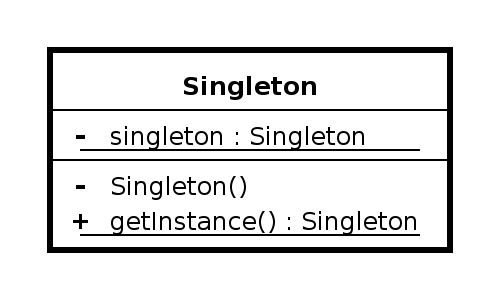
\includegraphics[scale=0.7]{SpecificaTecnica/Pics/Singleton}
        \caption{Struttura del pattern Singleton}
		\end{figure}
		Lo scopo del \insglo{pattern} creazionale denominato Singleton è 
		assicurare l'esistenza di un'unica istanza di una classe e fornire
		un punto di accesso globale ad essa.\\
		Questo \insglo{pattern} è nato per rispondere alla necessità di non avere più
		istanze della stessa classe, anche nei linguaggi in cui non è possibile 
		usare una variabile globale, pur dando la possibilità alla classe di
		tener traccia di quella sua istanza.\\
		Il \insglo{pattern} Singleton è quindi applicabile ogniqualvolta debba esistere una 
		sola istanza di una certa classe in tutta l'applicazione, prestando però attenzione 
		al fatto che l'istanza sia estendibile tramite ereditarietà.\\
		Viene generalmente utilizzato per implementare altri \insglo{pattern} come Factory, 
		Builder e Façade.
		\level{3}{Vantaggi nell'uso del Singleton}
		L'utilizzo del Singleton nell'implementazione di un \insglo{software} apporta i seguenti 
		vantaggi:
		\begin{itemize}
		\item controllo completo di come e quando i \insglo{client} accedono all'interfaccia;
		\item evita l'utilizzo ingiustificato di variabili globali;
		\item consente di ridefinire le operazioni definite nel Singleton;
		\item permette di porre un limite massimo al numero di istanze di una certa classe.
		\end{itemize}
	\level{2}{Dependency injection} \label{app:dependencyinjection}
Dependency Injection è un \insglo{pattern} architetturale utilizzato nella programmazione Object-Oriented il cui scopo è separare il comportamento di una componente dalla risoluzione delle sue dipendenze. \\
Questo particolare \insglo{pattern} si basa su tre elementi:
\begin{itemize}
\item una componente dipendente;
\item la dichiarazione delle dipendenze della componente, dette interface contracts;
\item un injector, detto anche provider, che crea su richiesta le istanze delle classi che implementano le dipendenze.
\end{itemize}
Il principio di programmazione adottato è quello dell'inversione di controllo, secondo il quale il ciclo di vita degli oggetti viene gestito da un'entità esterna (container).\\
Nel Dependency Injection implementato con l'inversione di controllo le dipendenze vengono inserite dal container, la componente si limita a dichiararle. In questo modo viene raggiunto l'obiettivo di ridurre le dipendenze fra classi.\\
Esistono due tipi di Dependency Injection:
\begin{description}
	\item[Constructor injection:] le dipendenze vengono dichiarate come parametri del costruttore; in questo modo un oggetto è valido appena viene istanziato.
	\item[Setter injection:] le dipendenze vengono dichiarate come metodi setter; in questo modo vengono evidenziate le dipendenze.
\end{description}

\level{3}{Vantaggi nell'uso di dependency injection}
L'utilizzo del \insglo{pattern} Dependency Injection nella progettazione dell'architettura di un \insglo{software} porta i seguenti vantaggi:
\begin{itemize}
\item la componente individuata come \insglo{client} è più facile da testare singolarmente attraverso l'uso di stub;
\item permette di esternalizzare i dettagli della configurazione del sistema in un file di configurazione, consentendo così di riconfigurare il sistema senza ricompilarlo;
\item permette lo sviluppo concorrente e indipendente del \insglo{software};
\item diminuisce l'accoppiamento tra una classe e la sua dipendenza.
\end{itemize}
\level{3}{Svantaggi nell'uso di dependency injection}
Dependency Injection ha anche delle possibili ripercussioni negative sul \insglo{software} che lo utilizza. Esso infatti può rendere il codice difficile da leggere in quanto permette la separazione fra dichiarazione e comportamento, oltre a richiedere più righe di codice rispetto alla scrittura di codice“tradizionale”per ottenere lo stesso comportamento.

	\level{2}{Observer} \label{app:observer}
		\begin{figure}[H]\centering
        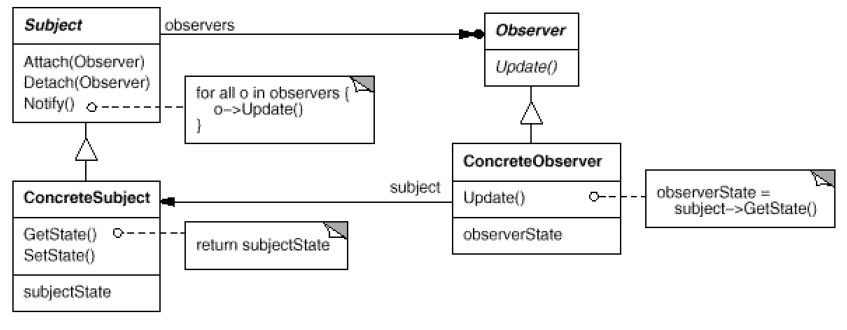
\includegraphics[scale=0.7]{SpecificaTecnica/Pics/Observer}
        \caption{Struttura del pattern Observer}
		\end{figure}
		Observer è un \insglo{pattern} comportamentale, implementato in numerose librerie di programmazione e sistemi, il cui scopo è quello di tenere sotto controllo lo stato di diversi oggetti legati ad un soggetto (dipendenza uno a molti). \\
		Il paradigma corrisponde al modello Publisher and Subscribe: i sottoscrittori si registrano presso un pubblicatore e quest’ultimo li informa ogni volta che ci sono nuove notizie (del genere sottoscritto).\\
		Il \insglo{pattern} è composto da:
		\begin{itemize}
		\item una classe astratta “Subject”, da cui eredita il soggetto concreto, che mantiene una lista di riferimenti agli oggetti dipendenti per poterli avvisare;
		\item Un’interfaccia “Observer” implementata dagli osservatori concreti, che tengono il riferimento al soggetto per poterne leggere lo stato.
		\end{itemize}
		\level{3}{Vantaggi nell’uso di observer}
			L’utilizzo del \insglo{pattern} Observer nella progettazione dell’architettura porta i seguenti vantaggi:
			\begin{itemize}
			\item minimizzazione dell’accoppiamento tra Observer e Subject, che possono essere usati indipendentemente gli uni dagli altri;
			\item aumento del grado di riuso dei singoli tipi;
			\item non si debbono fare assunzioni sugli oggetti dipendenti se si ha necessità di comunicare con loro;
			\item libertà di aggiungere osservatori dinamicamente alla lista, senza modificare il Subject.
			\end{itemize}

			\level{3}{Svantaggi nell'uso di Observer}
			L’utilizzo di Observer potrebbe causare:
			\begin{itemize}
			\item possibile cascata di notifiche: poiché gli observer mutuamente si ignorano, una richiesta di modifica può avere effetti incontrollati, scatenando la reazione degli altri;
			\item “memory leak” in quanto nelle implementazioni di base il subject richiede sia l’esplicita registrazione che l’esplicita rimozione dalla lista delle dipendenze legandosi in modo forte agli observer, tenendoli attivi. Questo problema può essere prevenuto riferendo in modo debole gli observer.
			\end{itemize}
\level{2}{Abstract Factory} \label{app:abstractfactory}
		\begin{figure}[H]\centering
        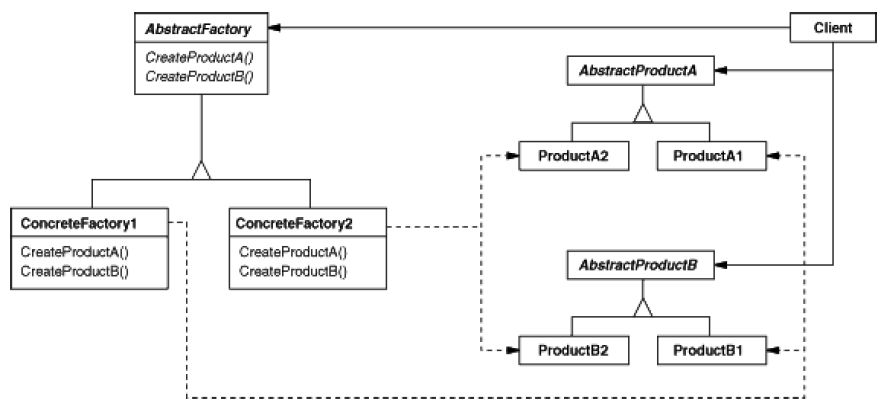
\includegraphics[scale=0.7]{SpecificaTecnica/Pics/AbstractFactory}
        \caption{Struttura del pattern Abstract Factory}
		\end{figure}
Abstract Factory è un \insglo{design pattern} creazionale utilizzato allo scopo di fornire un'interfaccia per la creazione di famiglie di prodotti, senza dover specificare classi concrete.\\
Il \insglo{pattern} si basa sui seguenti elementi:
\begin{description}
\item[AbstractFactory:] dichiara un'interfaccia per operazioni che creano prodotti astratti;
\item[ConcreteFactory:] implementa le operazioni per creare prodotti concreti;
\item[AbstractProduct:] dichiara un'interfaccia per un tipo di \insglo{prodotto};
\item[ConcreteProduct:] definisce un \insglo{prodotto} che deve creato dalla corrispondente factory concreta e implementa l'interfaccia di AbstractProduct.
\end{description}
La principale ragione per cui viene utilizzato questo \insglo{pattern} è la possibilità di rendere l'applicazione configurabile con diverse famiglie di prodotti. La flessibilità garantita dal \insglo{pattern} fa si che esso venga implementato ogniqualvolta:
\begin{itemize}
\item si voglia rendere il sistema indipendente dal modo in cui i suoi componenti sono creati;
\item si voglia rendere il sistema configurabile con più famiglie di prodotti;
\item le componenti di una famiglia debbano essere usate insieme;
\item si voglia fornire una libreria di classi \insglo{prodotto}, senza fornire informazioni circa la loro implementazione.
\end{itemize}
\level{3}{Vantaggi nell'uso di Abstract Factory}
L'impiego dell'Abstract Factory nella progettazione dell'architettura di un \insglo{prodotto} \insglo{software} porta i seguenti vantaggi:
\begin{itemize}
\item isolamento dei tipi concreti, in quanto ai \insglo{client} risultano visibili solo le interfacce dei prodotti, con la conseguenza di una maggiore flessibilità del \insglo{software};
\item maggiore semplicità nell'introdurre e usare diverse famiglie di prodotti;
\item favorisce la consistenza dei prodotti concreti.
\end{itemize}
\level{3}{Svantaggi nell'uso di Abstract Factory}
Come tutti i \insglo{pattern}, anche Abstract Factory ha delle ripercussioni negative nella progettazione del \insglo{software}: in questo caso risulta difficile estendere la classe factory astratta, perchè ciò comporta il cambiamento di tutte le sotto classi.

\level{2}{Adapter} \label{app:adapter}
	\begin{figure}[H]\centering
    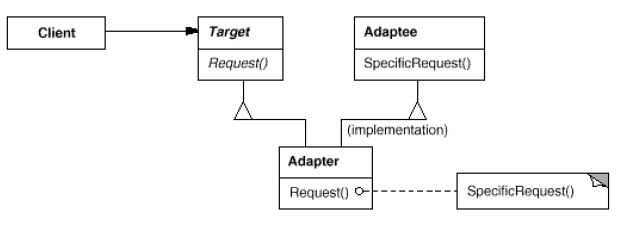
\includegraphics[scale=0.7]{SpecificaTecnica/Pics/ClassAdapter}
    \caption{Struttura del pattern Adapter nella versione ClassAdapter}
	\end{figure}
	\begin{figure}[H]\centering
    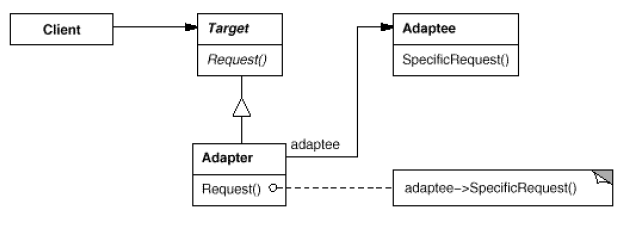
\includegraphics[scale=0.7]{SpecificaTecnica/Pics/ObjectAdapter}
    \caption{Struttura del pattern Adapter nella versione ObjectAdapter}
	\end{figure}
Adapter è un \insglo{pattern} strutturale che, come suggerisce il suo nome, viene utilizzato per adattare l'interfaccia di una classe in un'altra permettendo alle classi di lavorare assieme, cosa altrimenti non possibile.\\
Gli elementi del \insglo{pattern} sono:
\begin{description}
\item[Target:] è l'interfaccia di dominio, quella che di desidera mettere a disposizione del \insglo{Client};
\item[Adaptee:] è l'interfaccia esistente che si vuole adattare (ad esempio una libreria esterna);
\item[Adapter:] è la classe concreta che adatta Adaptee in Target.
\end{description}

Esso viene utilizzato ogni qualvolta sia necessario:
\begin{itemize}
\item utilizzare una classe esistente non conforme all'interfaccia Target;
\item creare classi riusabili anche con classi arbitrarie;
\item adattare un'interfaccia che non può essere adattata in altri modi.
\end{itemize}

Si può implementare questo \insglo{pattern} in due modi:
\begin{description}
\item[Class adapter:] in questo caso viene realizzata una classe concreta che implementa allo stesso tempo l'interfaccia esistente (quella da adattare) e l'interfaccia che si desidera per l'applicazione (detta interfaccia di dominio). Il vantaggio di questo metodo è che permette ad Adapter di modificare (anche estendendo) le caratteristiche di Adaptee; lo svantaggio è che non funziona quando bisogna adattare una classe alla base di una gerarchia;
\item[Object adapter:] in questo caso l'adattamento avviene sfruttando un campo dati del tipo dell'interfaccia da adattare all'interno della classe concreta; in questo modo l'interfaccia di dominio verrà implementata invocando i metodi dell'interfaccia Adaptee attraverso il campo dati. Il vantaggio di questo metodo è che permette ad Adapter di adattare più tipi; lo svantaggio è che non consente di modificare le caratteristiche dell'Adaptee.
\end{description}
Ne consegue che la scelta fra i due metodi va fatta in considerazione dell'uso che se ne vuole fare.

\level{2}{Bridge} \label{app:bridge}
	\begin{figure}[H]\centering
    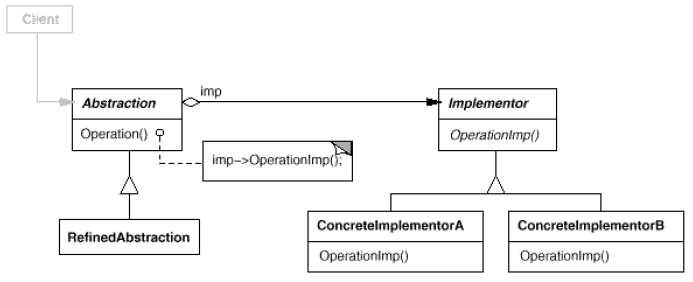
\includegraphics[scale=0.7]{SpecificaTecnica/Pics/Bridge}
    \caption{Struttura del pattern Bridge}
	\end{figure}
Bridge è un \insglo{pattern} strutturale che permette di separare l’interfaccia di una classe dalla sua implementazione. \\
Il \insglo{pattern} è composto da un’interfaccia che fa da ponte rendendo indipendenti le funzionalità della classe concreta dall’interfaccia che la implementa. Entrambe i tipi di classi possono essere modificati senza che questo causi problemi l’uno all’altro. \\
Viene utilizzato quando:
\begin{itemize}
\item si desidera evitare un binding permanente tra astrazione e interfaccia;
\item è necessario rendere estensibili tramite sub-classing astrazioni e implementazioni;
\item si vuole nascondere al \insglo{client} l'implementazione di un'astrazione;
\item si vuole condividere un'implementazione tra oggetti multipli nascondendo questo fatto al \insglo{client}.
\end{itemize}

\level{3}{Vantaggi nell’uso di Bridge}
L’utilizzo del \insglo{pattern} Bridge nella progettazione dell’architettura porta i seguenti vantaggi:
\begin{itemize}
\item maggiore estensibilità data dalla possibilità di estendere indipendentemente le gerarchie delle interfacce e delle classi che le implementano;
\item mascheramento dei dettagli implementativi permesso dall'implementazione nascosta delle interfacce.
\end{itemize}
